\scanpage{4}
\mspage{3}

\textcircled{\scriptsize c}\quad $\forall\,T\in\mathrm{Modf}(\mathcal L)$, et $A\in C(T)/R_T$
une classe suivant $R_T$, une partie
de $\dot A\subset T$, appelée \uline{frontière} de $A$.

Ces données \textcircled{\scriptsize a} \textcircled{\scriptsize b}, \textcircled{\scriptsize c} étant \unsure{assujetties}
à satisfaire certains axiomes.

Je prévois que les axiomes impliquent
\deleted{Soit \illegible{1} $\unsure{t|U}\in C(T)$, \unsure{on pose}}
ceci

1°) que la donnée \textcircled{\scriptsize c} résulte déjà de \textcircled{\scriptsize b}

2°) que la donnée \textcircled{\scriptsize b} résulte de
la donnée des $R_T$, \deleted{\unsure{pour}} dans le cas
particulier où $T\in S_0$. Donc
les seules \unsure{donnée|données} essentielles \unsure{serait|seraient}
\textcircled{\scriptsize a} \unsure{celles|celle} des 0-sphères i.e. la notion
de \deleted{pos.} lieux en pos. relative modérée
(condition \inserted{réflexive et} symétrique) et \textcircled{\scriptsize b} La donnée,
pour \figure{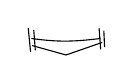
\begin{tikzpicture}[x=1cm,y=1cm,baseline=-.4ex]
\draw (0,.12)--(.03,-.18) (0.07,.10)--(.09,-.16);
\draw (.90,.12)--(.92,-.15) (.96,.09)--(.97,-.12);
\draw (.04,-.01) to[out=-8,in=187] (.92,-.01);
\draw (.05,-.10)--(.48,-.22)--(.94,-.06);
\end{tikzpicture}} $\varepsilon\in S_0$, de la relation
d'équivalence $R_{\varepsilon}$ dans $C(\varepsilon)$.

\deleted{On va} \uline{Axiomes provisoires :}

\deleted{Soit $X$} Appellons les $U$ de la forme
$C(\deleted{\unsure{L}}T)$ \uline{parties modérées cofinies}. On

% paper watermark
\rotatebox{90}{\textsc{\unsure{Strong Extra St}}}
